\documentclass[a4paper, 12pt, notitlepage]{article}
\usepackage[margin=0.5in]{geometry}
\usepackage[english]{babel}
\usepackage[utf8x]{inputenc}
\usepackage{fancyhdr}
\usepackage{amsmath}
\usepackage{amssymb}
\usepackage{gensymb}
\usepackage[makeroom]{cancel}
\usepackage{newfloat}
\usepackage{pdfpages}
\usepackage{graphicx}
\usepackage{tabularx}
\usepackage{hyperref}

\title{Computational Biology - 1$^\text{st}$ Assignment}
\author{Nicolás Espinoza Muñoz}
\date{October 3, 2020}

\newcommand\numberthis{\addtocounter{equation}{1}\tag{\theequation}}
\pagenumbering{gobble}

\begin{document}
\maketitle
\subsubsection*{Introduction}
This text presents the simulation work developed as part of the first assignment of the course in Computational Biology I. It is separated into two parts, corresponding to two sets of simulations. The first of these is related to a group of interacting Harmonic Oscillators - the interaction consists of an energetic one, further explained in the corresponding section.\\\\
The second part reviews the simulation of a real Ideal Gas. That is to say, particles posses only kinetic energy, but can interact with one another through collisions mediated by an artifact called Maxwell daemon.\\\\
\section*{Harmonic Oscillator}
In this first section, all simulations concern a number of harmonic oscillators that interact with one another by means of energy transference. Independently of the initial distribution of the energy over the array of oscillators, the program selects any two of them at random, and attempts a reduction of energy on one of them, and a corresponding energy increase of the same magnitude on the other, thus simulating an energy transfer process; the attempt fails if the giving oscillator's energy drops below 0 as a result of the interaction. The program outputs two files: The first one, \texttt{hist.dat}, is the probability, that the first oscillator has of being found in a certain normalized energy state. The second file, \texttt{entropy.dat}, is the entropy of the whole system as a function of the number of energy transference attempts between two oscillators.\\\\
For starters, we will check what the probability distribution on the first oscillator looks like, and whether this is consistent across simulations with different input parameters. This distribution corresponds to the amount of time - equivalent in this context to how many simulation steps - said oscillator is found to be in a given energetic state, and how the two main variables (number of oscillators $N$ and system energy $E$) affect the simulation. Next we will explore the probability distribution, and find the fitting constant for some of the simulations attempted. Finally we present the difference between initial energy distributions and how both evolve over simulation cycles to reach a common maximum system entropy value. Also together with this analysis, we show that entropy has a direct dependence on the amount of elements that conform the system.\\\\
As a final note before proceeding to the proper experiments, we show in Figure \ref{fig:fig1} that there is no significant dependence on the number of cycles, at least for the intended purposes of this assignment. Therefore, using $1.000.000$ simulation cycles is accepted as a value which balances calculation time and precision.
\begin{figure}[h]
	\begin{minipage}{0.5\textwidth}
		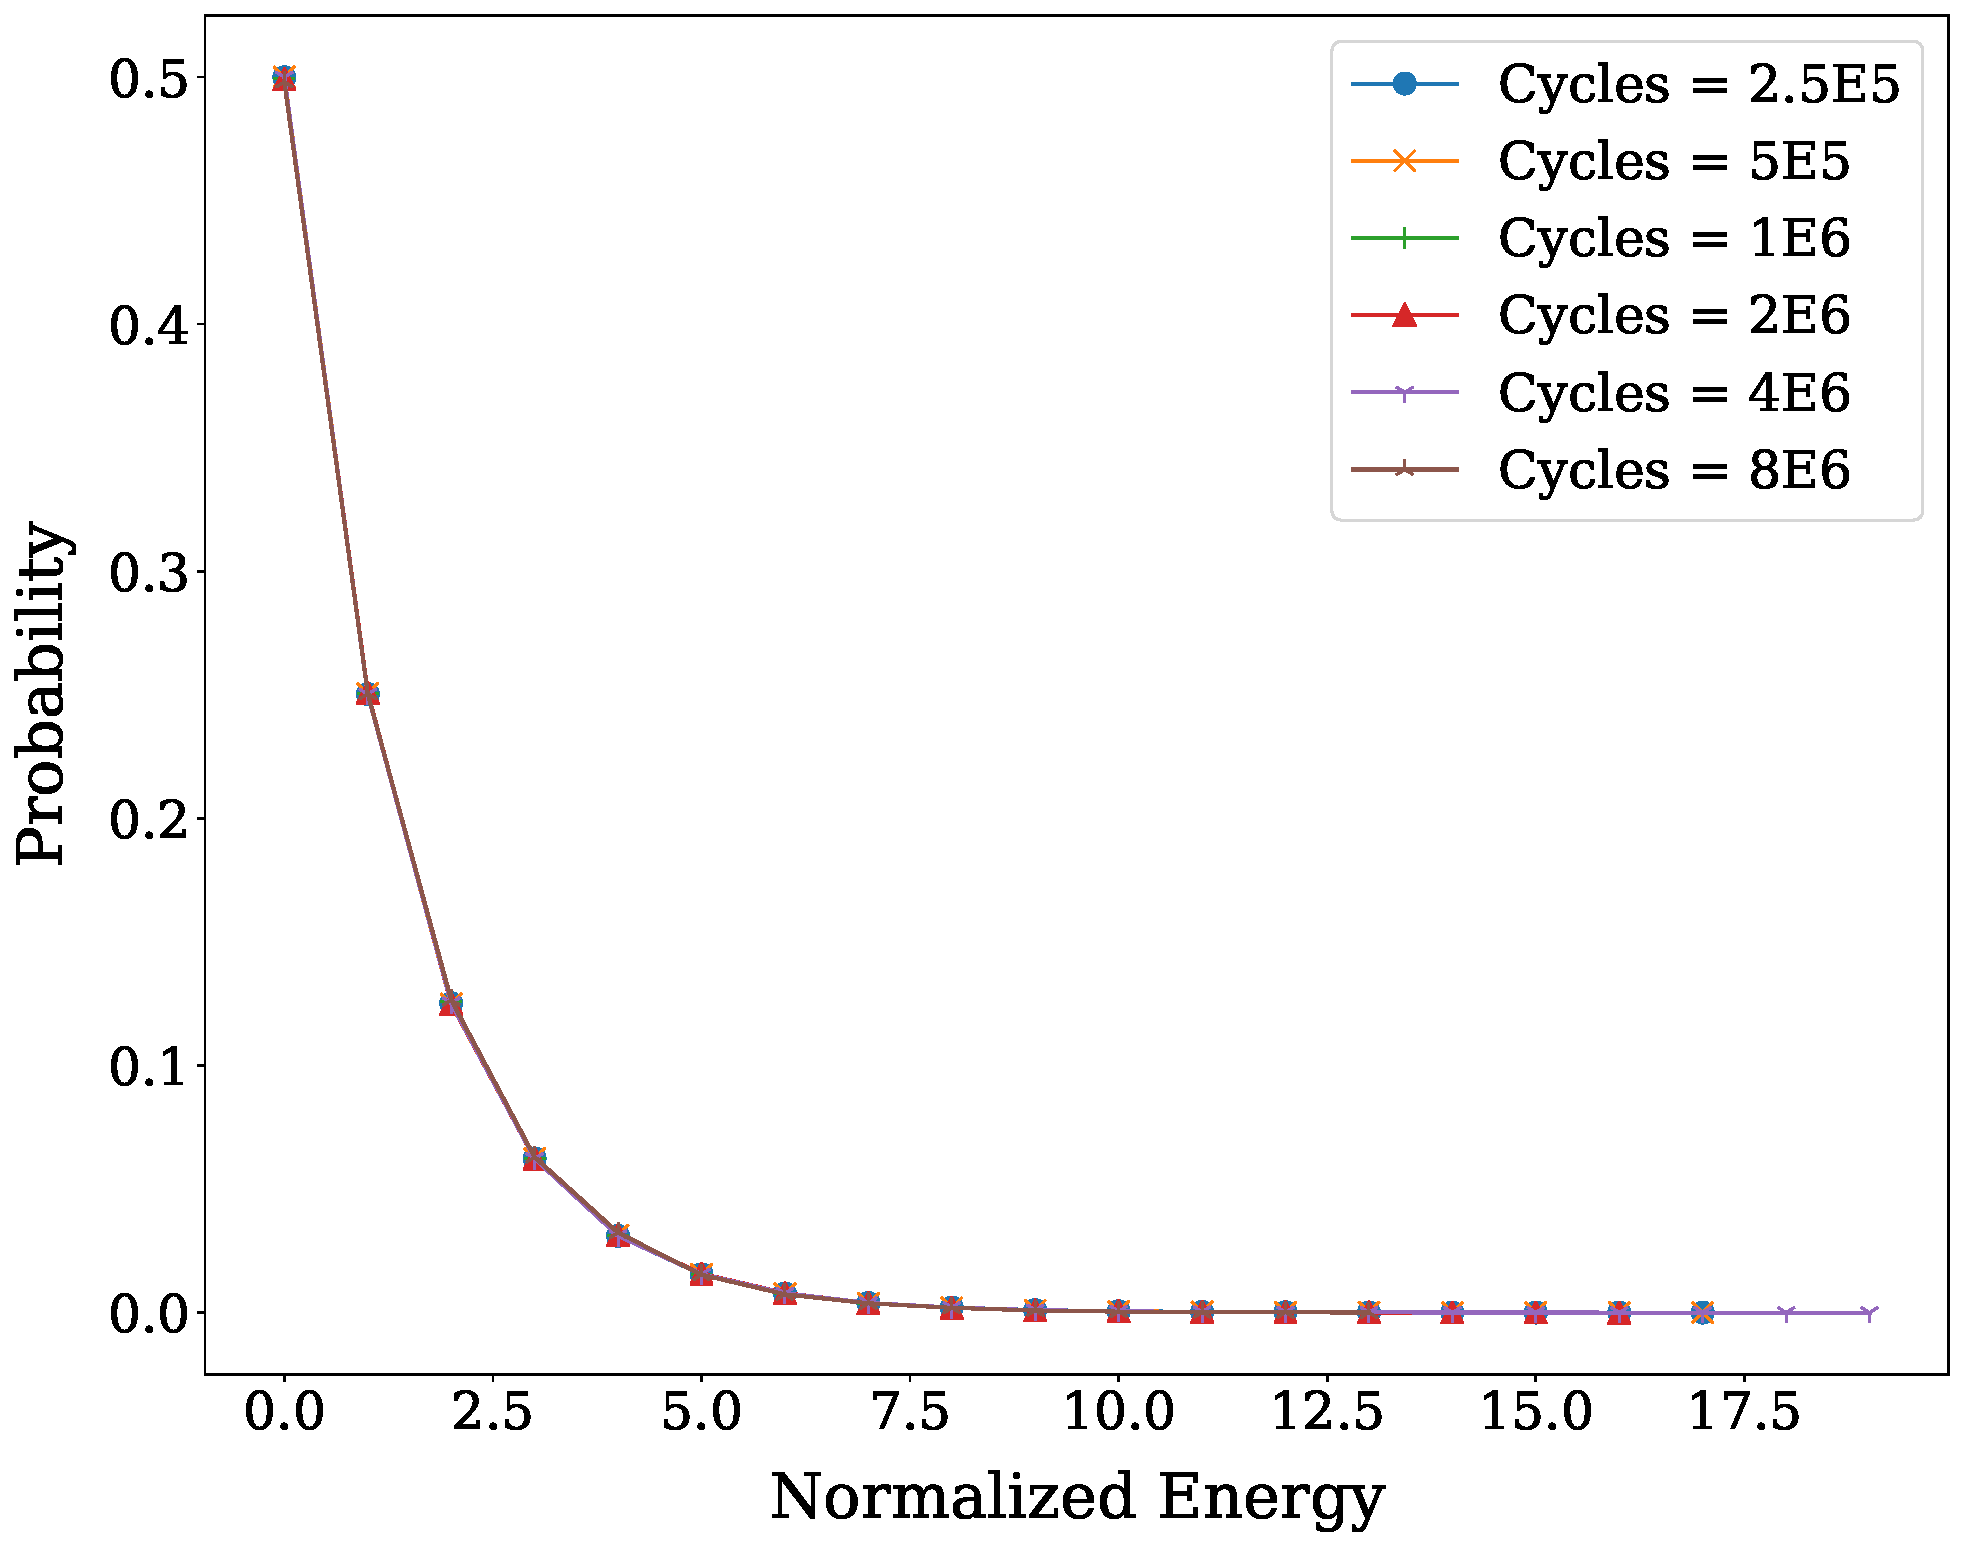
\includegraphics[scale = 0.27]{./Figs/convergence.pdf}
	\end{minipage}
	\begin{minipage}{0.3\textwidth}
		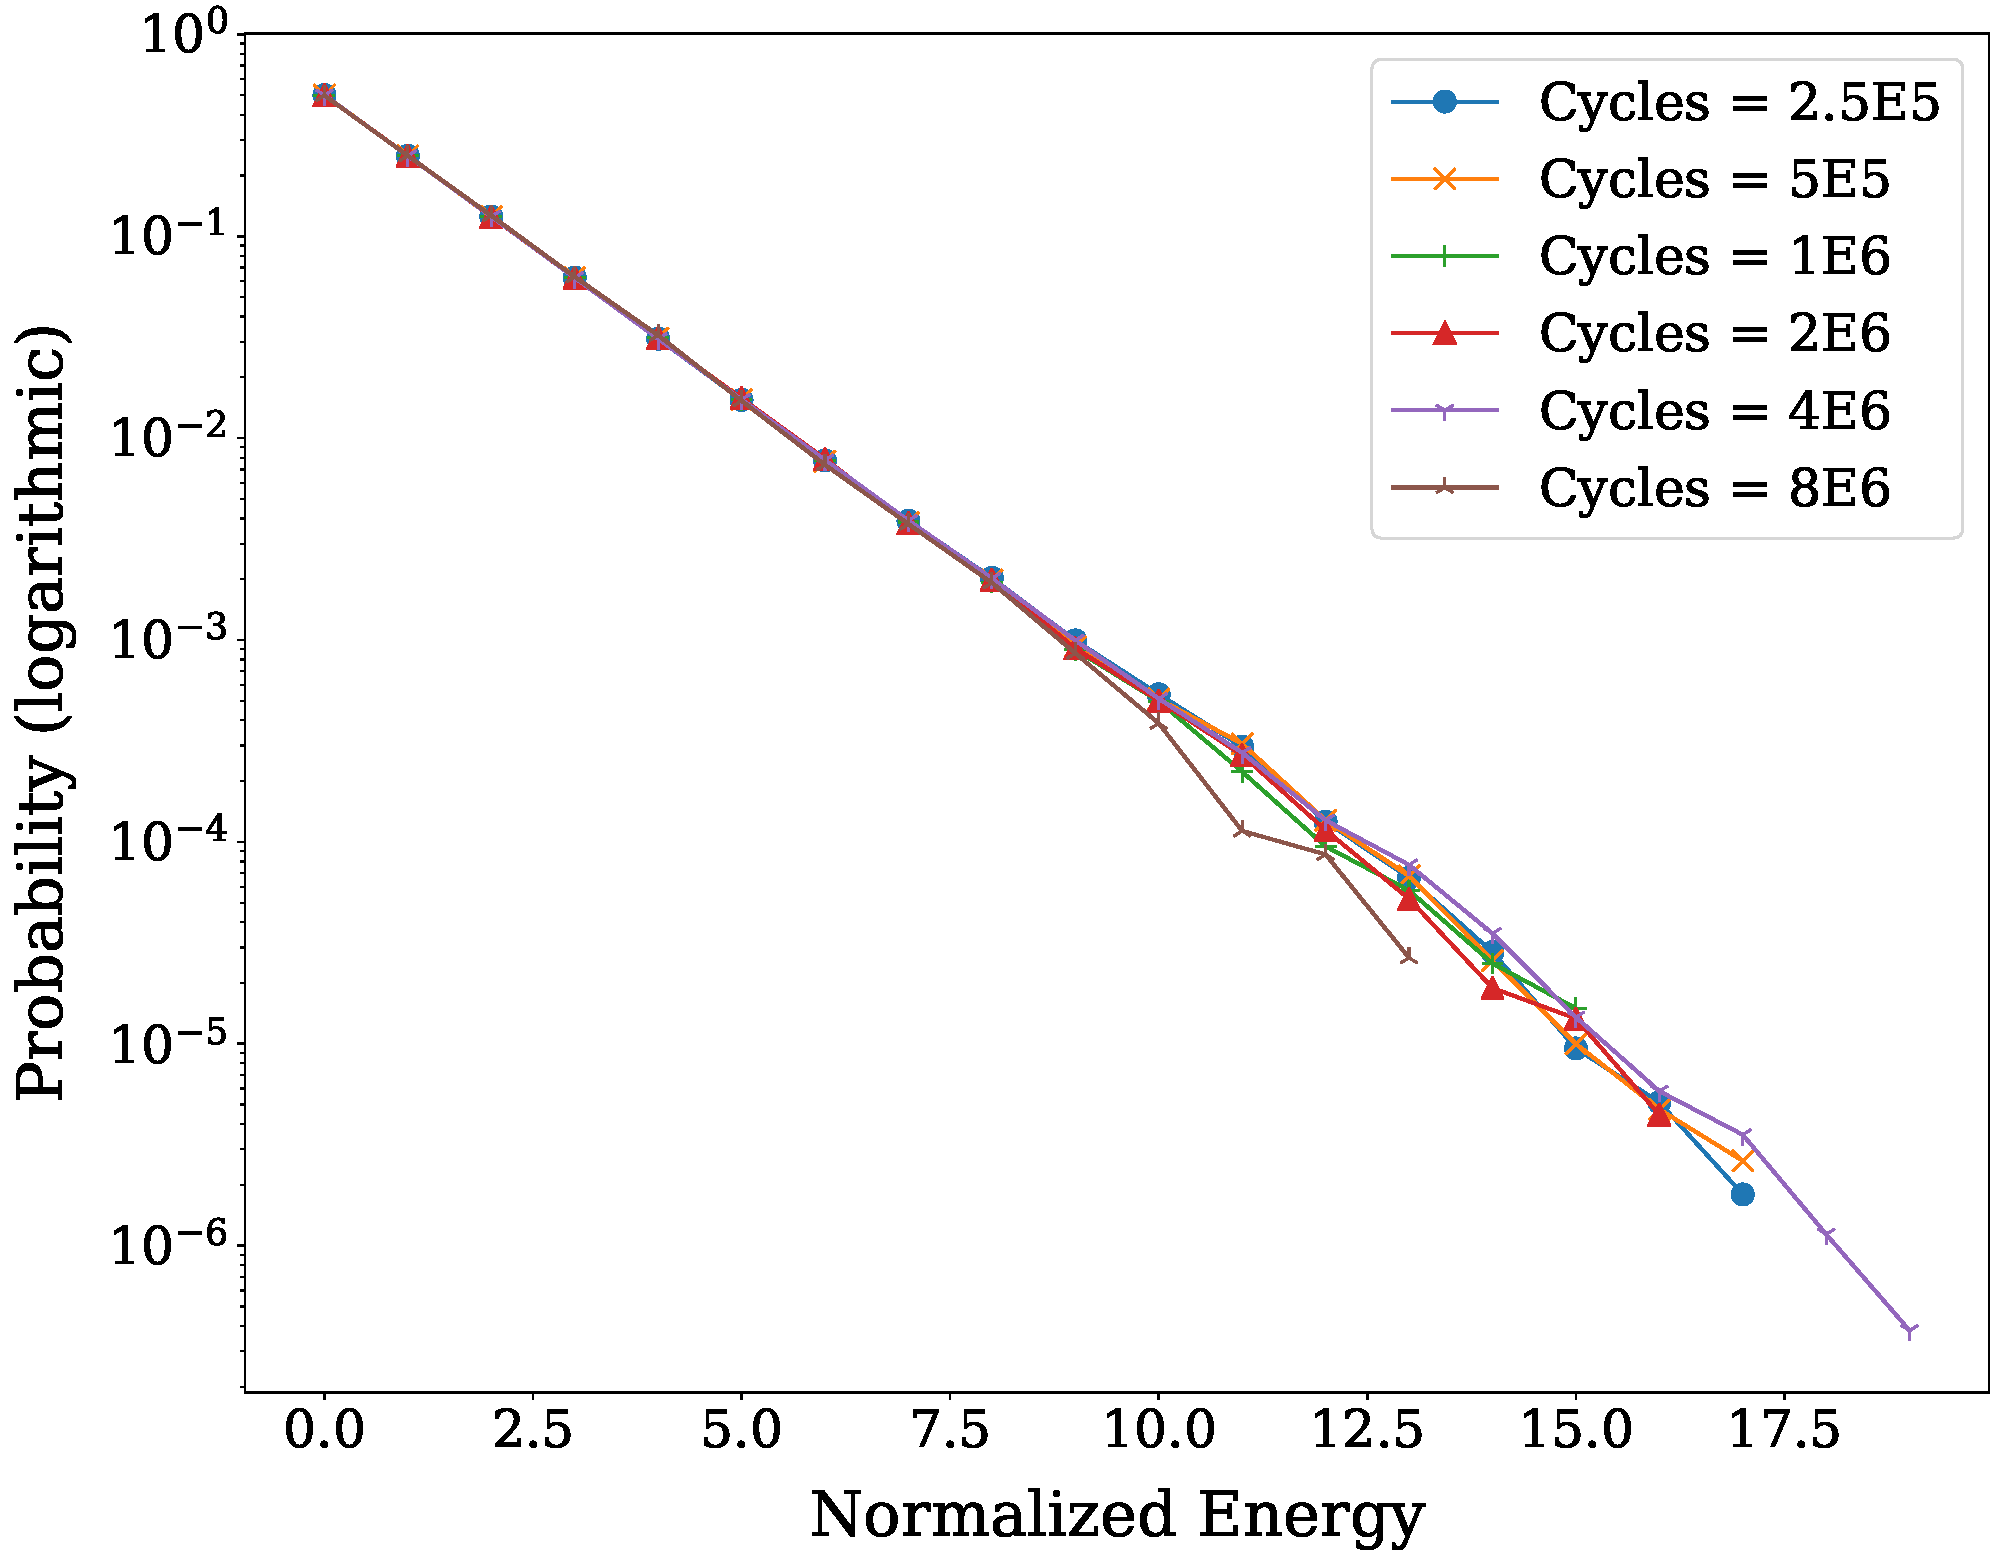
\includegraphics[scale = 0.27]{./Figs/Convergence-log.pdf}
	\end{minipage}
\caption{Convergence of the energy values of the first oscillator for different amounts of cycles. This was tested for $E=10000$ and $N=10000$.}\label{fig:fig1}
\end{figure}

\subsubsection*{Probability as function of $N$ and $E$}
In this experiment we dug into the importance of the two mentioned parameters in the simulation results, specifically the probability distribution of the first particle. Results in the next figure show that, although there are changes, the distribution itself continues to be a decaying exponential. The calculations were made for a fixed number of elements $N = 5000$.

\begin{figure}[h]
	\centering
	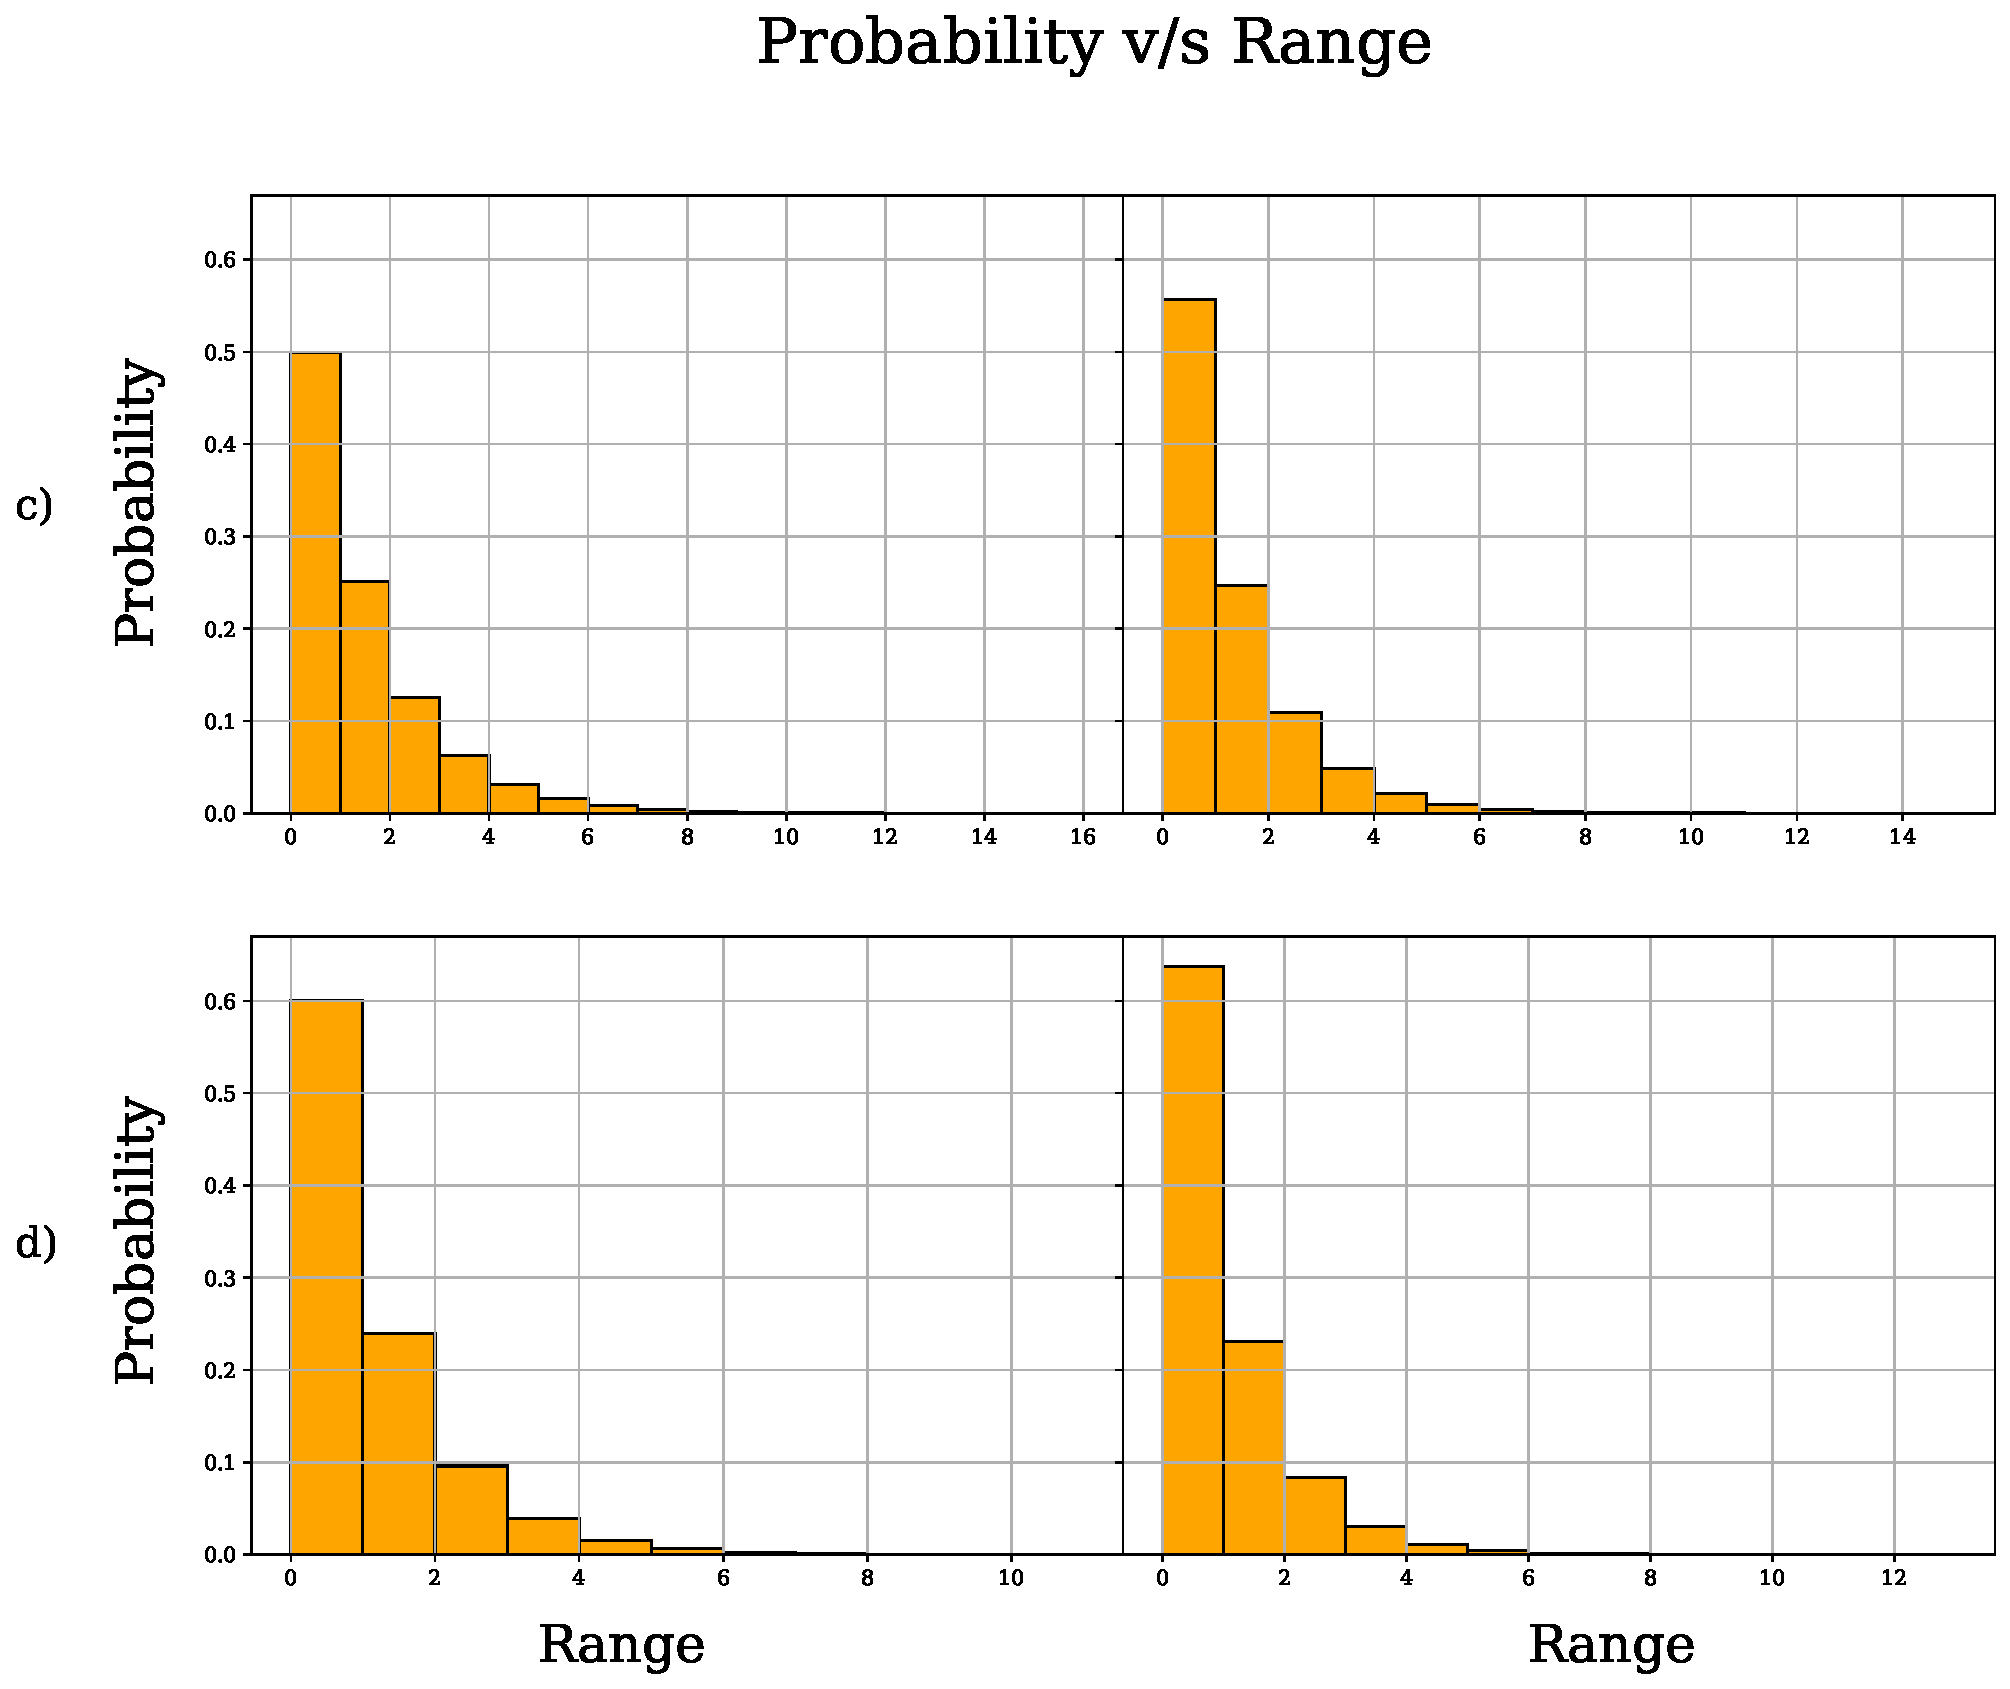
\includegraphics[scale = 0.4]{./Figs/P3/plots-1.pdf}
	\caption{Probability of the first oscillator to be found in the range of normalized energy states presented in the $X$ axes of the histograms. From left to right: a) $E = 5000$ and $E = 7500$, b) $E = 10000$ and $E = 12500$.}\label{fig:fig2}
\end{figure}

\noindent
We can see that, apart from some kind of hiccup in the first histogram of Figure \ref{fig:fig2} b), which is normal as this is a probabilistic process, the results are really consistent. The differences between distributions can be explained by considering that each subsequent graph describes a system with more energy than the one before, so it's only natural that all oscillators have a higher chance of spending more cycles in states of higher energy. For example, comparing the first and last histograms, we see that the last one is more evenly distributed, and in that system the first oscillator has a much higher probability of being found in states of let's say energy 10, whereas in the graph of the first system it pretty much has no chance of reaching that energy level, and most probably it was detected at that energy value when transferring energy to the other oscillators\footnote{In the first step of the simulation, all energy packages are given to the first oscillator.}.\\\\
In the next set of histograms we tested a fixed energy value $E = 10000$, and tried different amounts of oscillators. The results are presented in Figure \ref{fig:fig3}

\begin{figure}[!h]
	\centering
	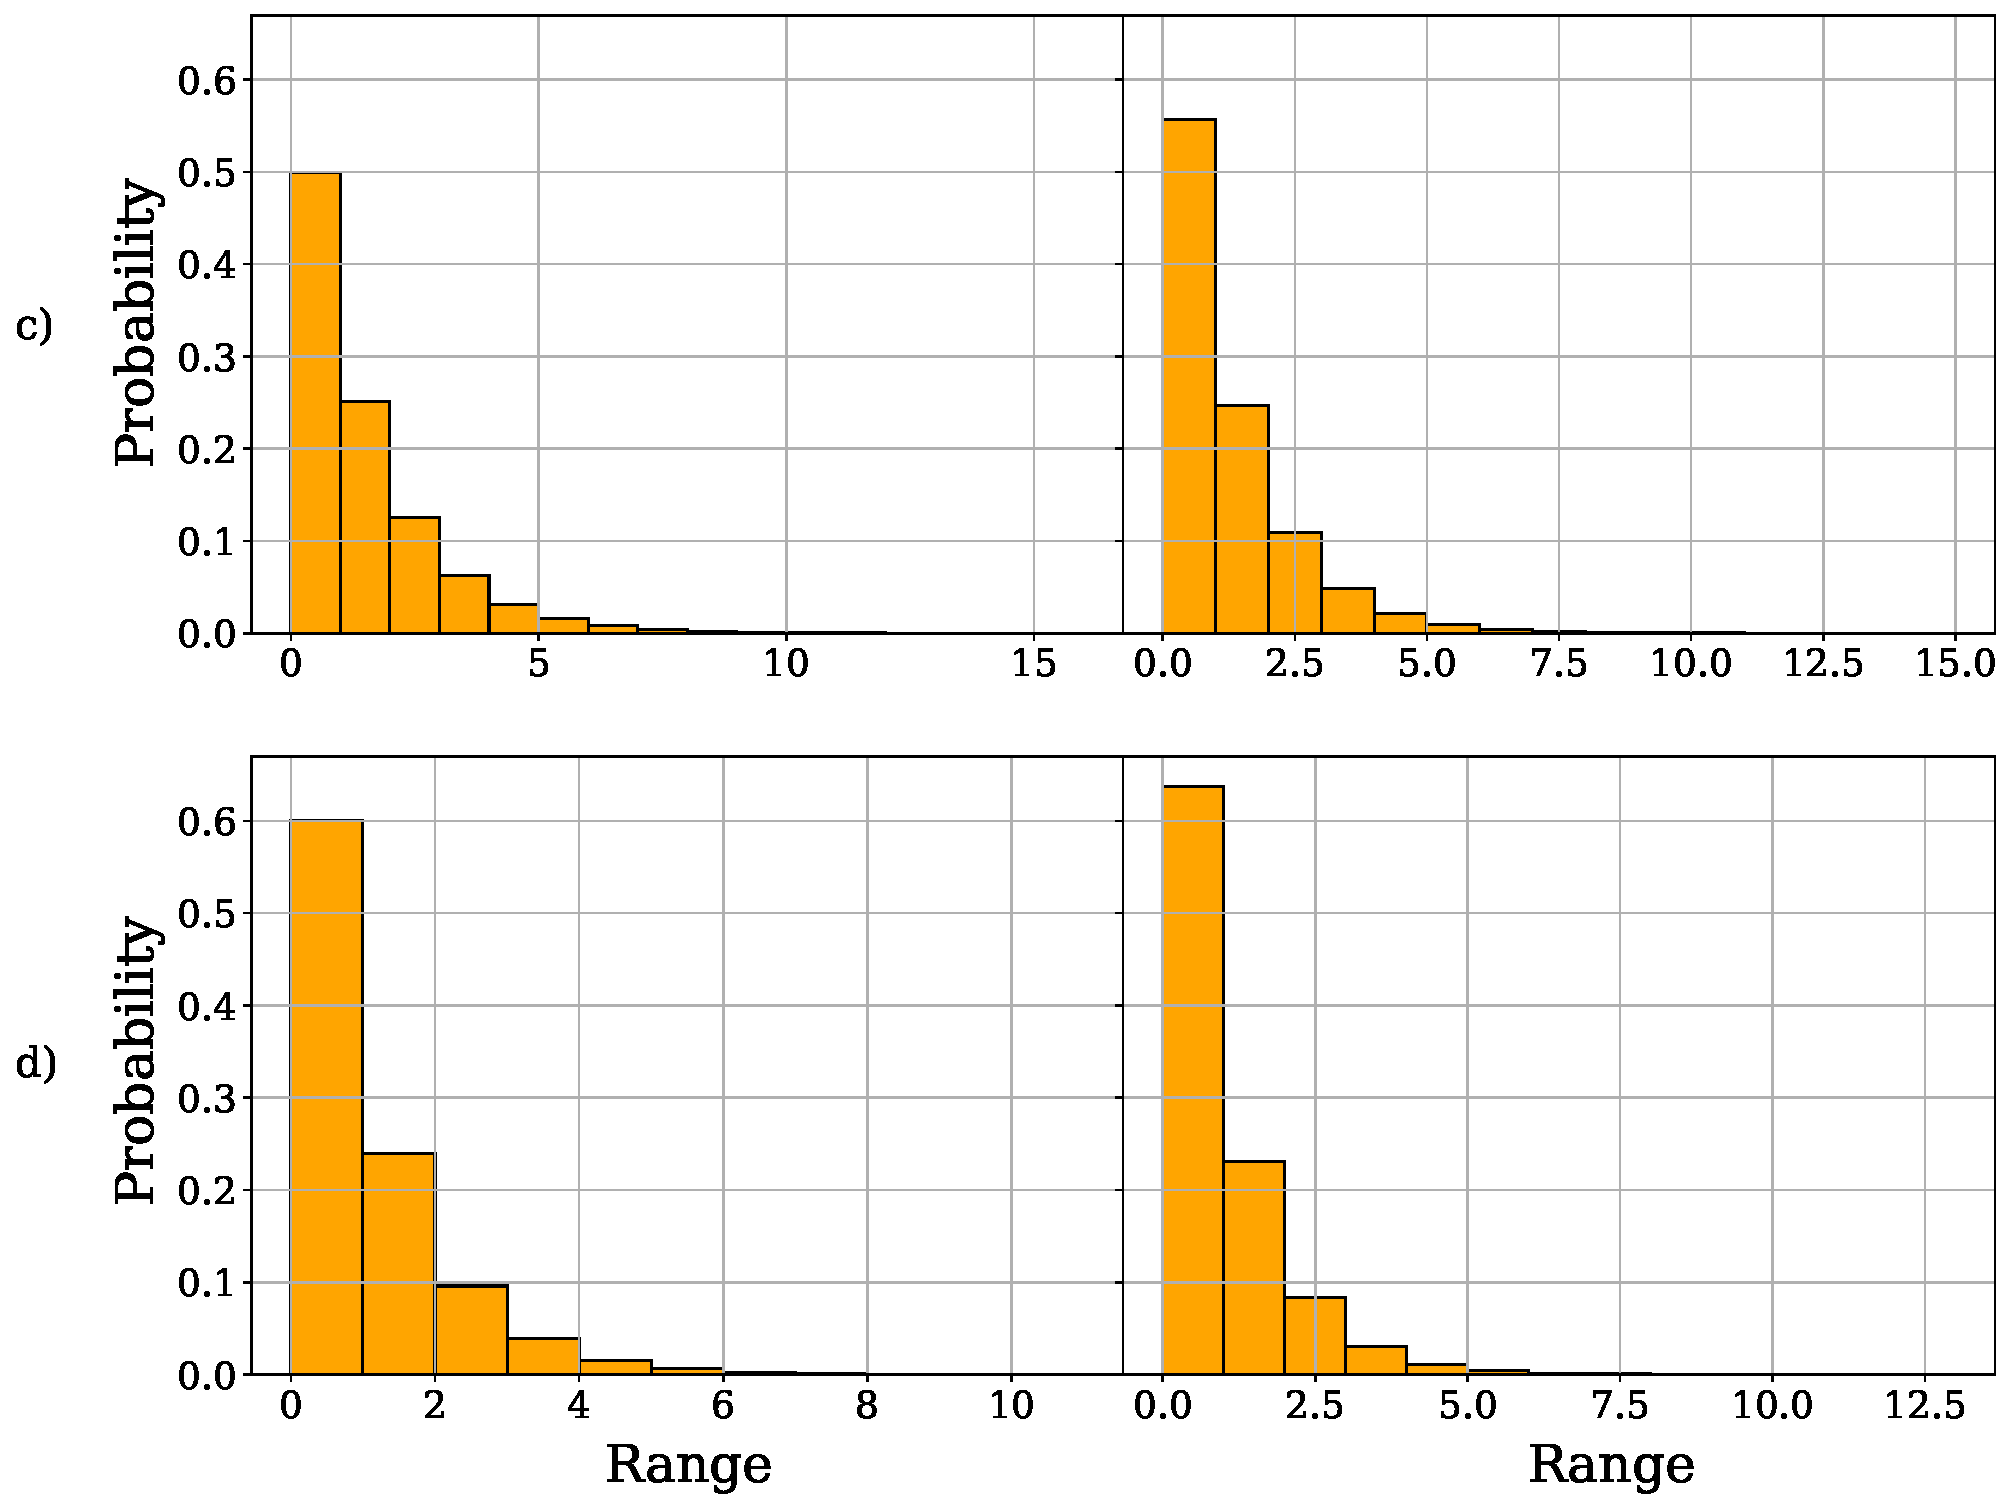
\includegraphics[scale=0.4]{./Figs/P3/plots-2.pdf}
	\caption{Akin to Figure \ref{fig:fig2}, this set, from left to right, presents systems with: c) $N = 10000$ and $N = 12500$, and d) $N = 15000$ and $17500$.}\label{fig:fig3}
\end{figure}

\noindent
It's clear that when having a 1:1 ratio of energy and oscillators in a system, the probability distribution is pretty much the same for all of them. We once again find in Figure \ref{fig:fig3} that a higher total energy means the first oscillator will spend more cycles in higher energy states. This can be directly concluded, as in the eight histograms shown by now, the probability of finding the first oscillator in low energy values gets higher as the ratio $E/N$ gets lower. That is to say, the system naturally tries to reach an even distribution of energy among all elements.

\subsubsection*{Obtaining the $\beta$ and $Q$ factors}
We can already see that the probability distribution is exponential, of the form $(Q^{-1})\cdot e^{-\beta k}$. We now proceed to determine the unknowns $Q$ and $\beta$ by applying the logarithm function:
\begin{align}
	P(k) =& \left.\frac{1}{Q}e^{-\beta\cdot k}\qquad\qquad\right/\ln\label{eq:1} \\
	\ln (P(k)) =& -\ln(Q) - \beta\cdot k\label{eq:2}
\end{align}
This makes it possible to determine the unknown values following the same procedure as if it were a straight line equation. After fitting via Ordinary Least Squares method, we can go back from step (\ref{eq:2}) to (\ref{eq:1}) to recover the exponential form.\\\\
We show in Figure \ref{fig:fig4} the fitting together with the original (exponential) version of the probability expression. For space's sake, only the linear versions of corresponding systems from Figure \ref{fig:fig3} are presented, but the process is the same for any and every system.
\begin{figure}[h]
	\centering
	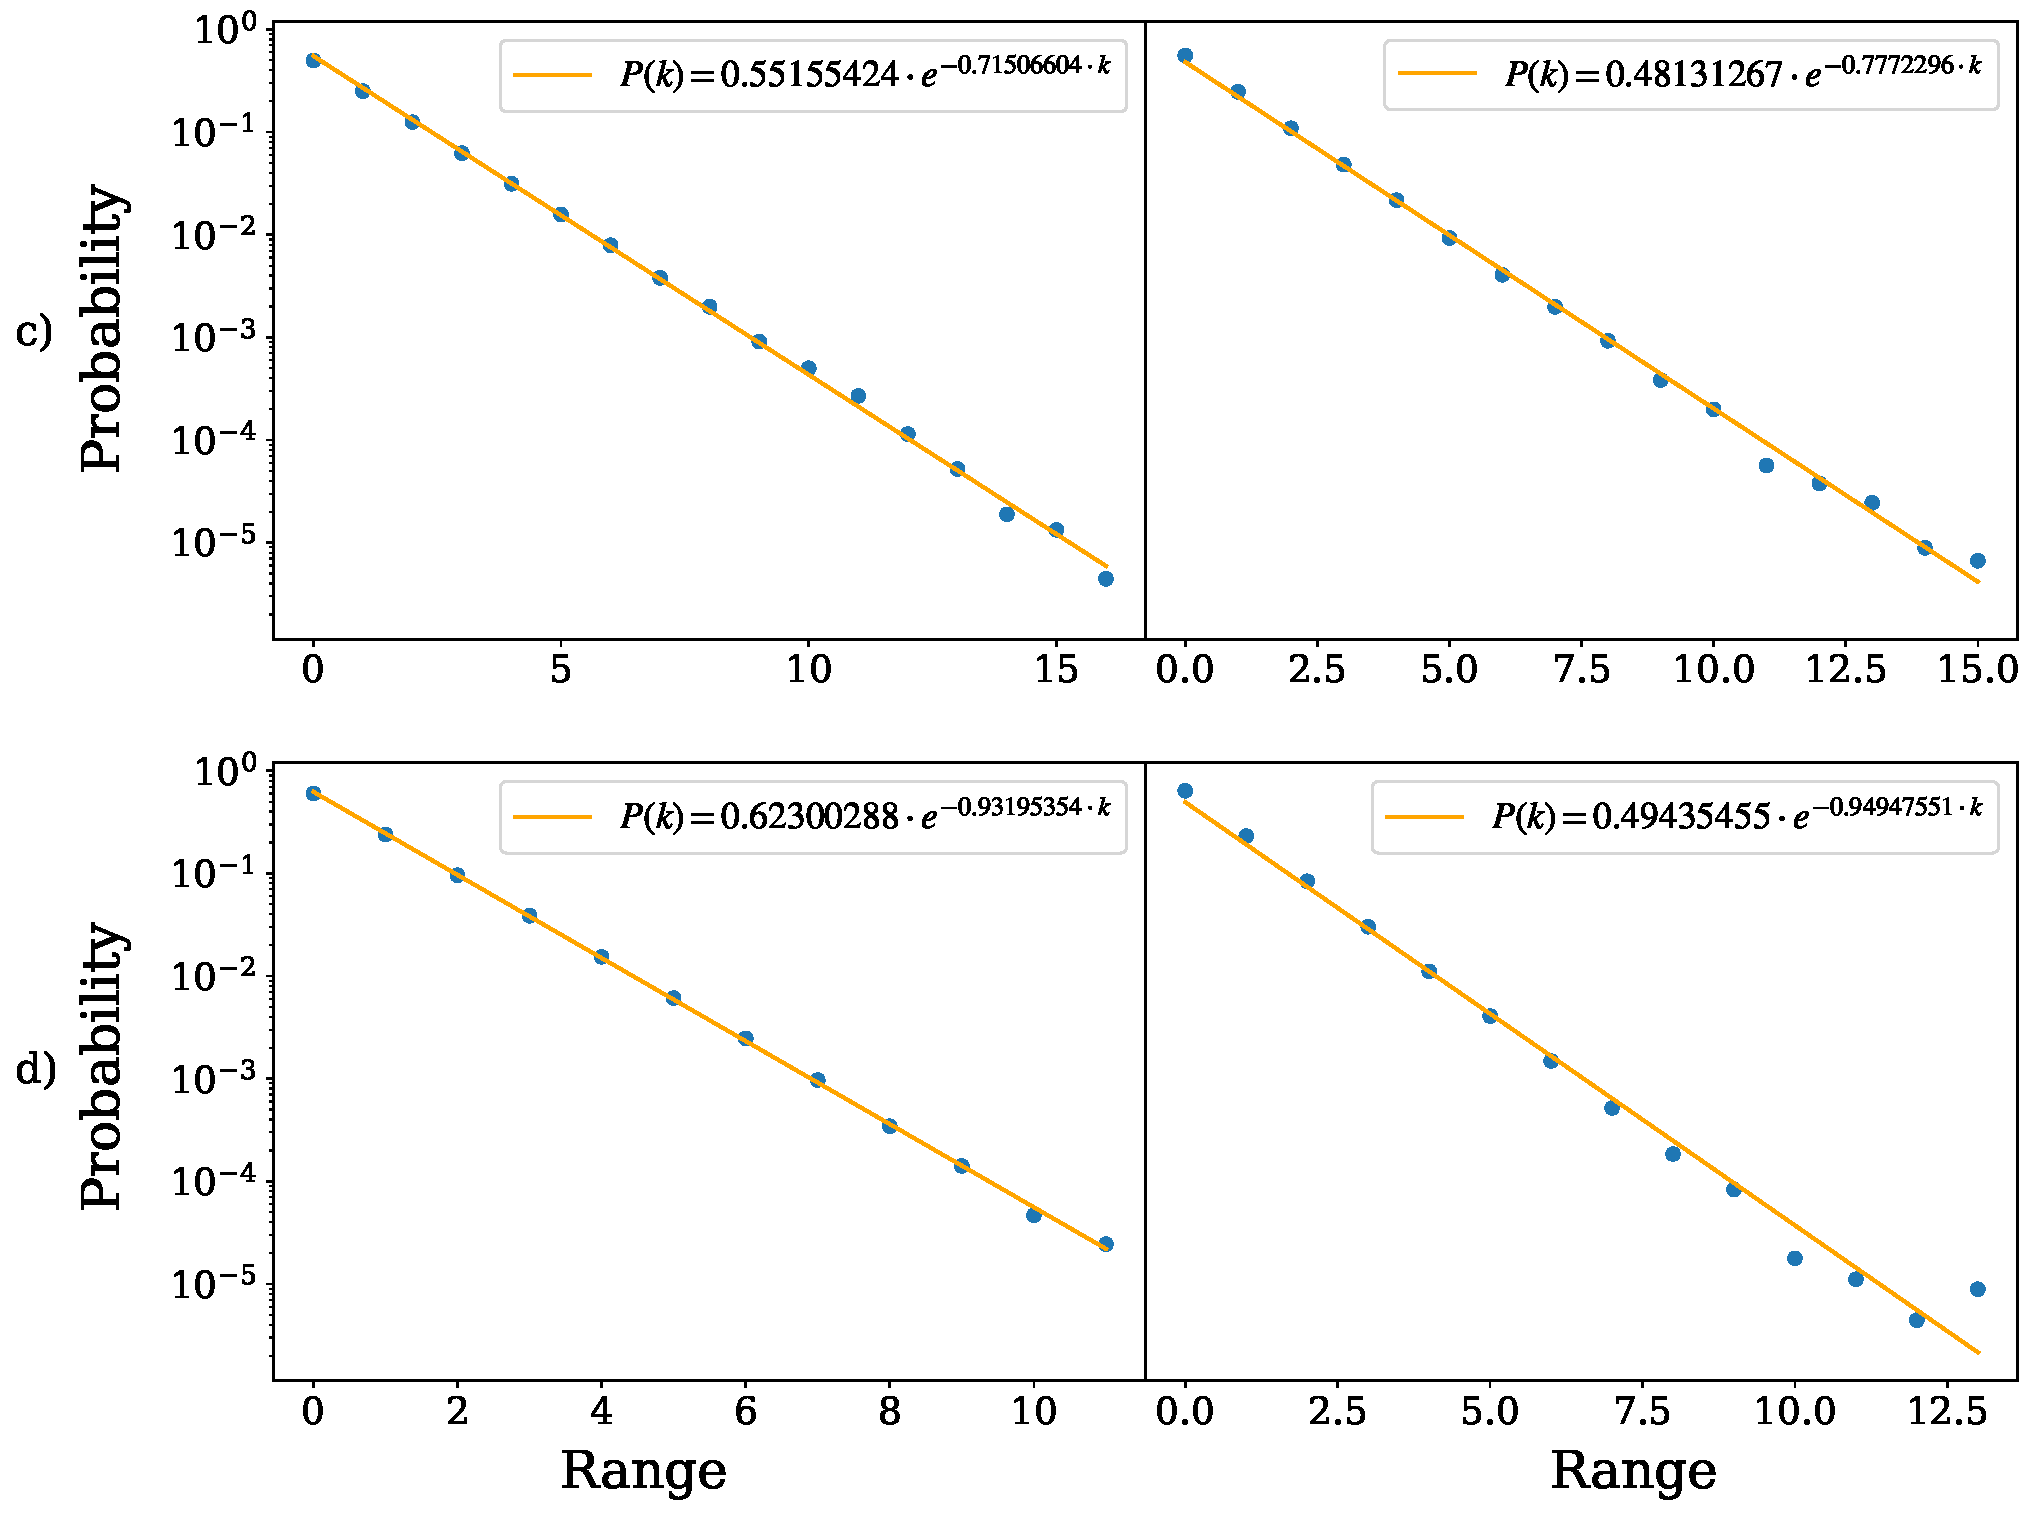
\includegraphics[scale=0.39]{./Figs/P3/plots-linear.pdf}
	\caption{Logarithmic probability for systems c) and d). The values of $\beta$ and $1/Q$ are presented in the legends of each plot.}\label{fig:fig4}
\end{figure}
Also we can see that for higher energy levels ($k$), the probability of the oscillator (and any oscillator) of being in that energy state decreases exponentially, with systems with less energy or more oscillators decaying faster for reasons explained in the previous section. We have to point out that in a normalized energy case, like these, $1/Q = 1$. Imprecision arise because we are fitting a curve to an exponential function, and a small deviation is therefore heavily accentuated. That is the main reason why the factor accompanying the exponential term in each fit is different from 1.

\subsubsection*{Entropy of the system}
As a last section of this first part of the work, we mess with the entropy of the system by altering the initial energy distribution, as well as the initial energy value and number of oscillators (not all at once).
\begin{figure}[h]
	\centering
	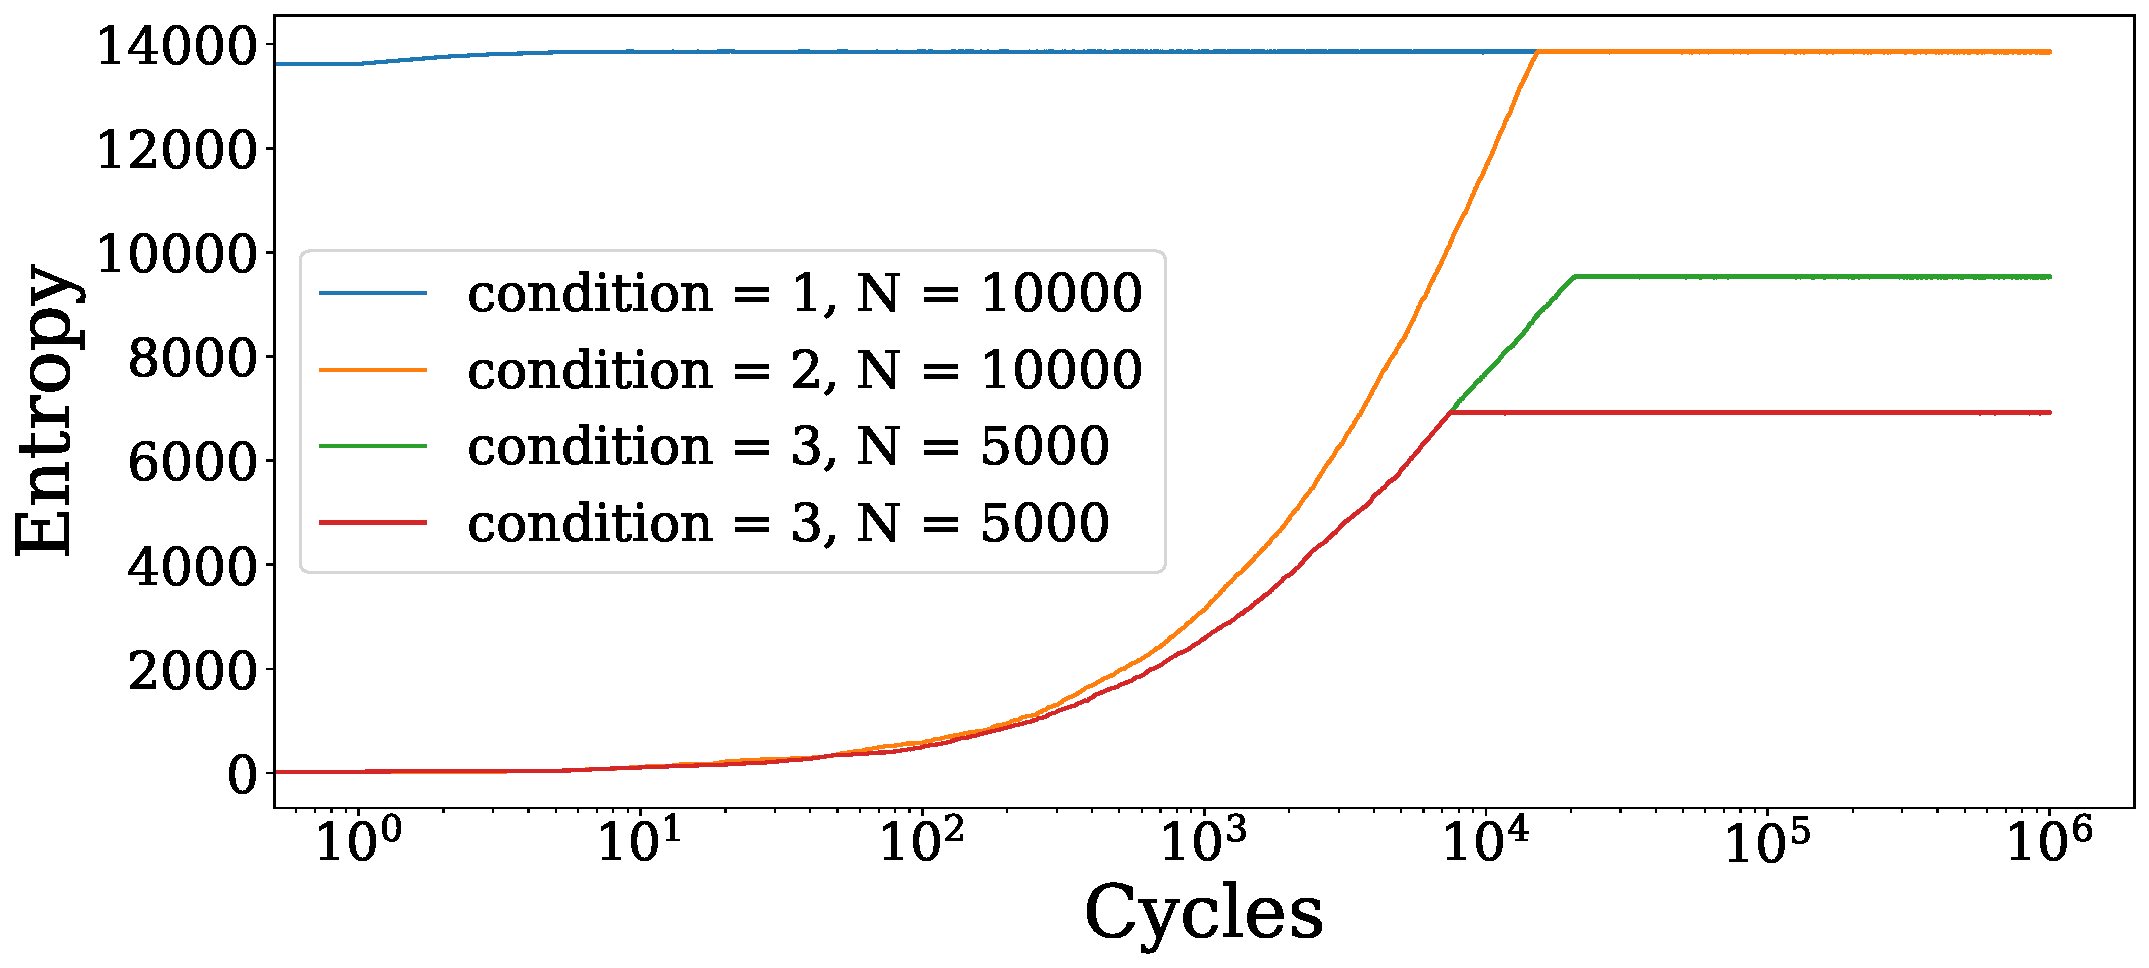
\includegraphics[scale=0.4]{./Figs/P4.pdf}
	\caption{Plot of the entropy as a function of cycle count (logarithmic scale for cycle count). The plots in blue, orange and green have 10000 energy packages, but the red one has just 5000.}\label{fig:fig5}
\end{figure}
The first thing to note is that, given enough time or attempts, the system's entropy will reach a maximum regardless of the initial energy distribution (orange line). However, the initial step's entropy is a fraction above 0 when all energy packages are given to the first oscillator, which makes sense because there is just a handful\footnote{This is, relatively speaking} of configurations possible were one oscillator has all the energy of the system. Conversely, there are a lot of possible combinations for more evenly distributions of the energy (blue line in Figure \ref{fig:fig5}), and since entropy is a function of the multiplicity of the system - in this cases its states - it gets higher as more configurations become available with the simulation progression.\\\\
From the plot we can also see that for a system with less elements, the entropy reaches a maximum far lower (green line). That is because there are fewer accessible configurations, as the number of oscillators is lower. Last, the red line shows us a system with half the entropy of the blue and orange ones. That is consistent, as the red system has both half the energy and half the number of oscillators as the systems with highest entropy, so it is basically a half system. Even though entropy is a logarithmic function of the number of states, the fact that it's entropy is halved makes sense in the context of harmonic oscillators, because of the nature of the interactions simulated.
\section*{Ideal Gas}
We begin this second part by showing that the energy of an ideal gas, which depends on parameters in a quadratic fashion, is not conserved when subjected to a change in one of the quantum numbers of two particles, one decreasing and one increasing.
\begin{align*}
	\mathbf{n}_1 = (2,2,3) \quad\rightarrow\quad \mathbf{n}_1* = (2,2,2)\\
	\mathbf{n}_2 = (1,1,1) \quad\rightarrow\quad \mathbf{n}_2* = (1,1,2)
\end{align*}
Knowing that the energy of a particle is given by
\begin{equation*}
	E_\mathbf{n} = \frac{h^2}{8mL^2}\left[n_x^2 + n_y^2 + n_z^2\right]
\end{equation*}
We calculate both the energy lost by $\mathbf{n}_1$ and won by $\mathbf{n}_2$
\begin{gather*}
	E_{\mathbf{n}_1} = \frac{h^2}{8mL^2}\left[2^2 + 2^2 + 3^2\right] = 17\cdot\frac{h^2}{8mL^2} \quad \rightarrow \quad \frac{h^2}{8mL^2}\left[2^2 + 2^2 + 2^2\right] = 12\cdot\frac{h^2}{8mL^2}\\[10pt]
	\therefore\quad \Delta E_{\mathbf{n}_1} = \boxed{-5}\\[10pt]
	E_{\mathbf{n}_2} = \frac{h^2}{8mL^2}\left[1^2 + 1^2 + 1^2\right] = 3\cdot\frac{h^2}{8mL^2} \quad \rightarrow \quad \frac{h^2}{8mL^2}\left[1^2 + 1^2 + 2^2\right] = 6\cdot\frac{h^2}{8mL^2}\\[10pt]
	\therefore\quad \Delta E_{\mathbf{n}_2} = \boxed{3}\\[10pt]
	\implies \quad \Delta E_{\mathbf{n}_2} \neq \Delta E_{\mathbf{n}_1}
\end{gather*}
So to keep energy constant, the use of an intermediate step is necessary. The Maxwell daemon takes care of the energy transference, acting as an energetic reservoir of sorts. When an attempted reduction in one of a particle's quantum numbers (and the corresponding increase in another particle's numbers) prompts the system to lose energy, this difference is instead kept by the daemon, which then returns the energy stored if another interaction would make the system gain more than what is available.\footnote{A more elaborate explanation can be found in M Creutz. Microcanonical Monte Carlo Simulation. \textit{Phys.Rev.Lett}, 50:1411, 1983. or in Harvey Gould and Jan Tobochnik. \textit{Statistical and Thermal Physics}. Princeton Universiy Press, USA, 2011.}\\\\
We simulate a system of real ideal gas particles - ideal gas particles that collide with one another - and make use of the Maxwell daemon to make it conservative. The idea is to show that, since the dependence of the energy is on three numbers, a specific energy state has more than one corresponding set of quantum numbers. In other words, there is more than one way to get a specific energy value. Thus, the resulting histogram of the energy states of the first particle is as follows
\begin{figure}[h]
	\centering
	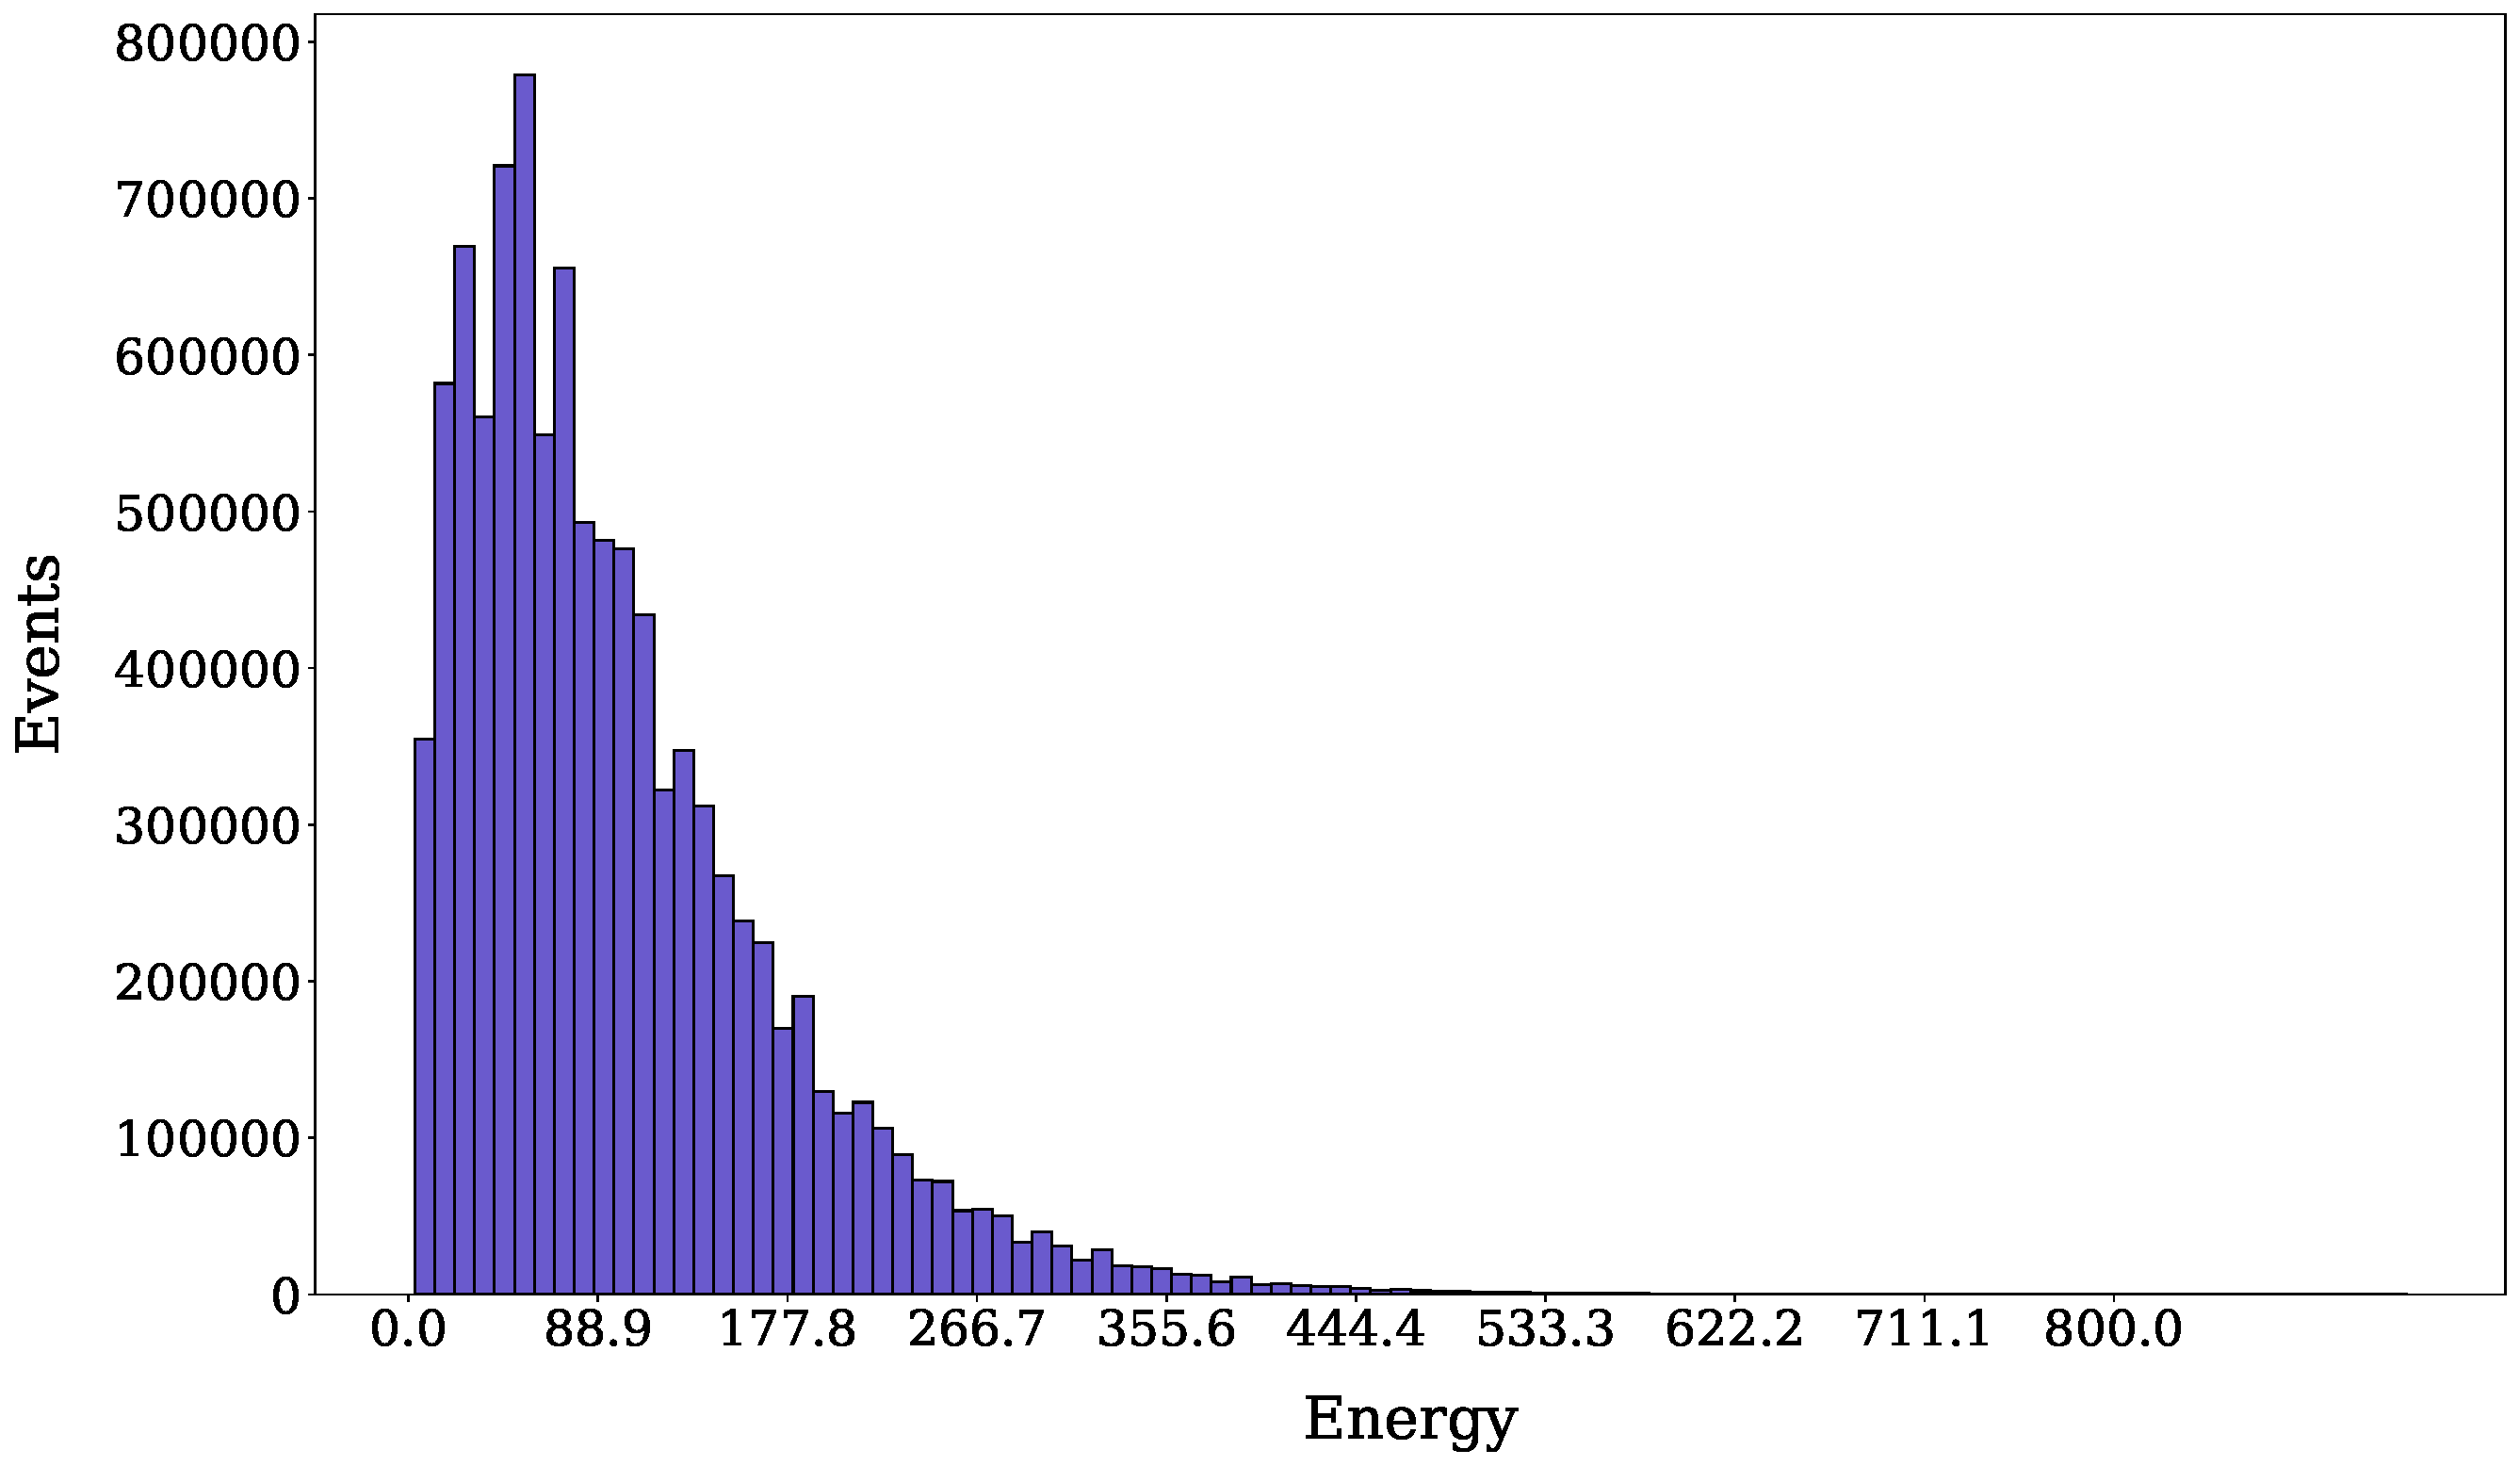
\includegraphics[scale=0.33]{./Figs/IG-hist.pdf}
	\caption{This graph shows that the energy of the first particle cannot be fitted by an exponential function on its own.}\label{fig:fig6}
\end{figure}

\noindent
The energy distribution shown in Figure \ref{fig:fig6} appears to be more of a piecewise function, decaying as an exponential only after it achieved its peak value (in the graphic, not in terms of energy value). Next we present the scatter plot of the first particle's energy as a function of the cycle - the system's attempts to transfer energy between particles.
\begin{figure}[!h]
	\centering
	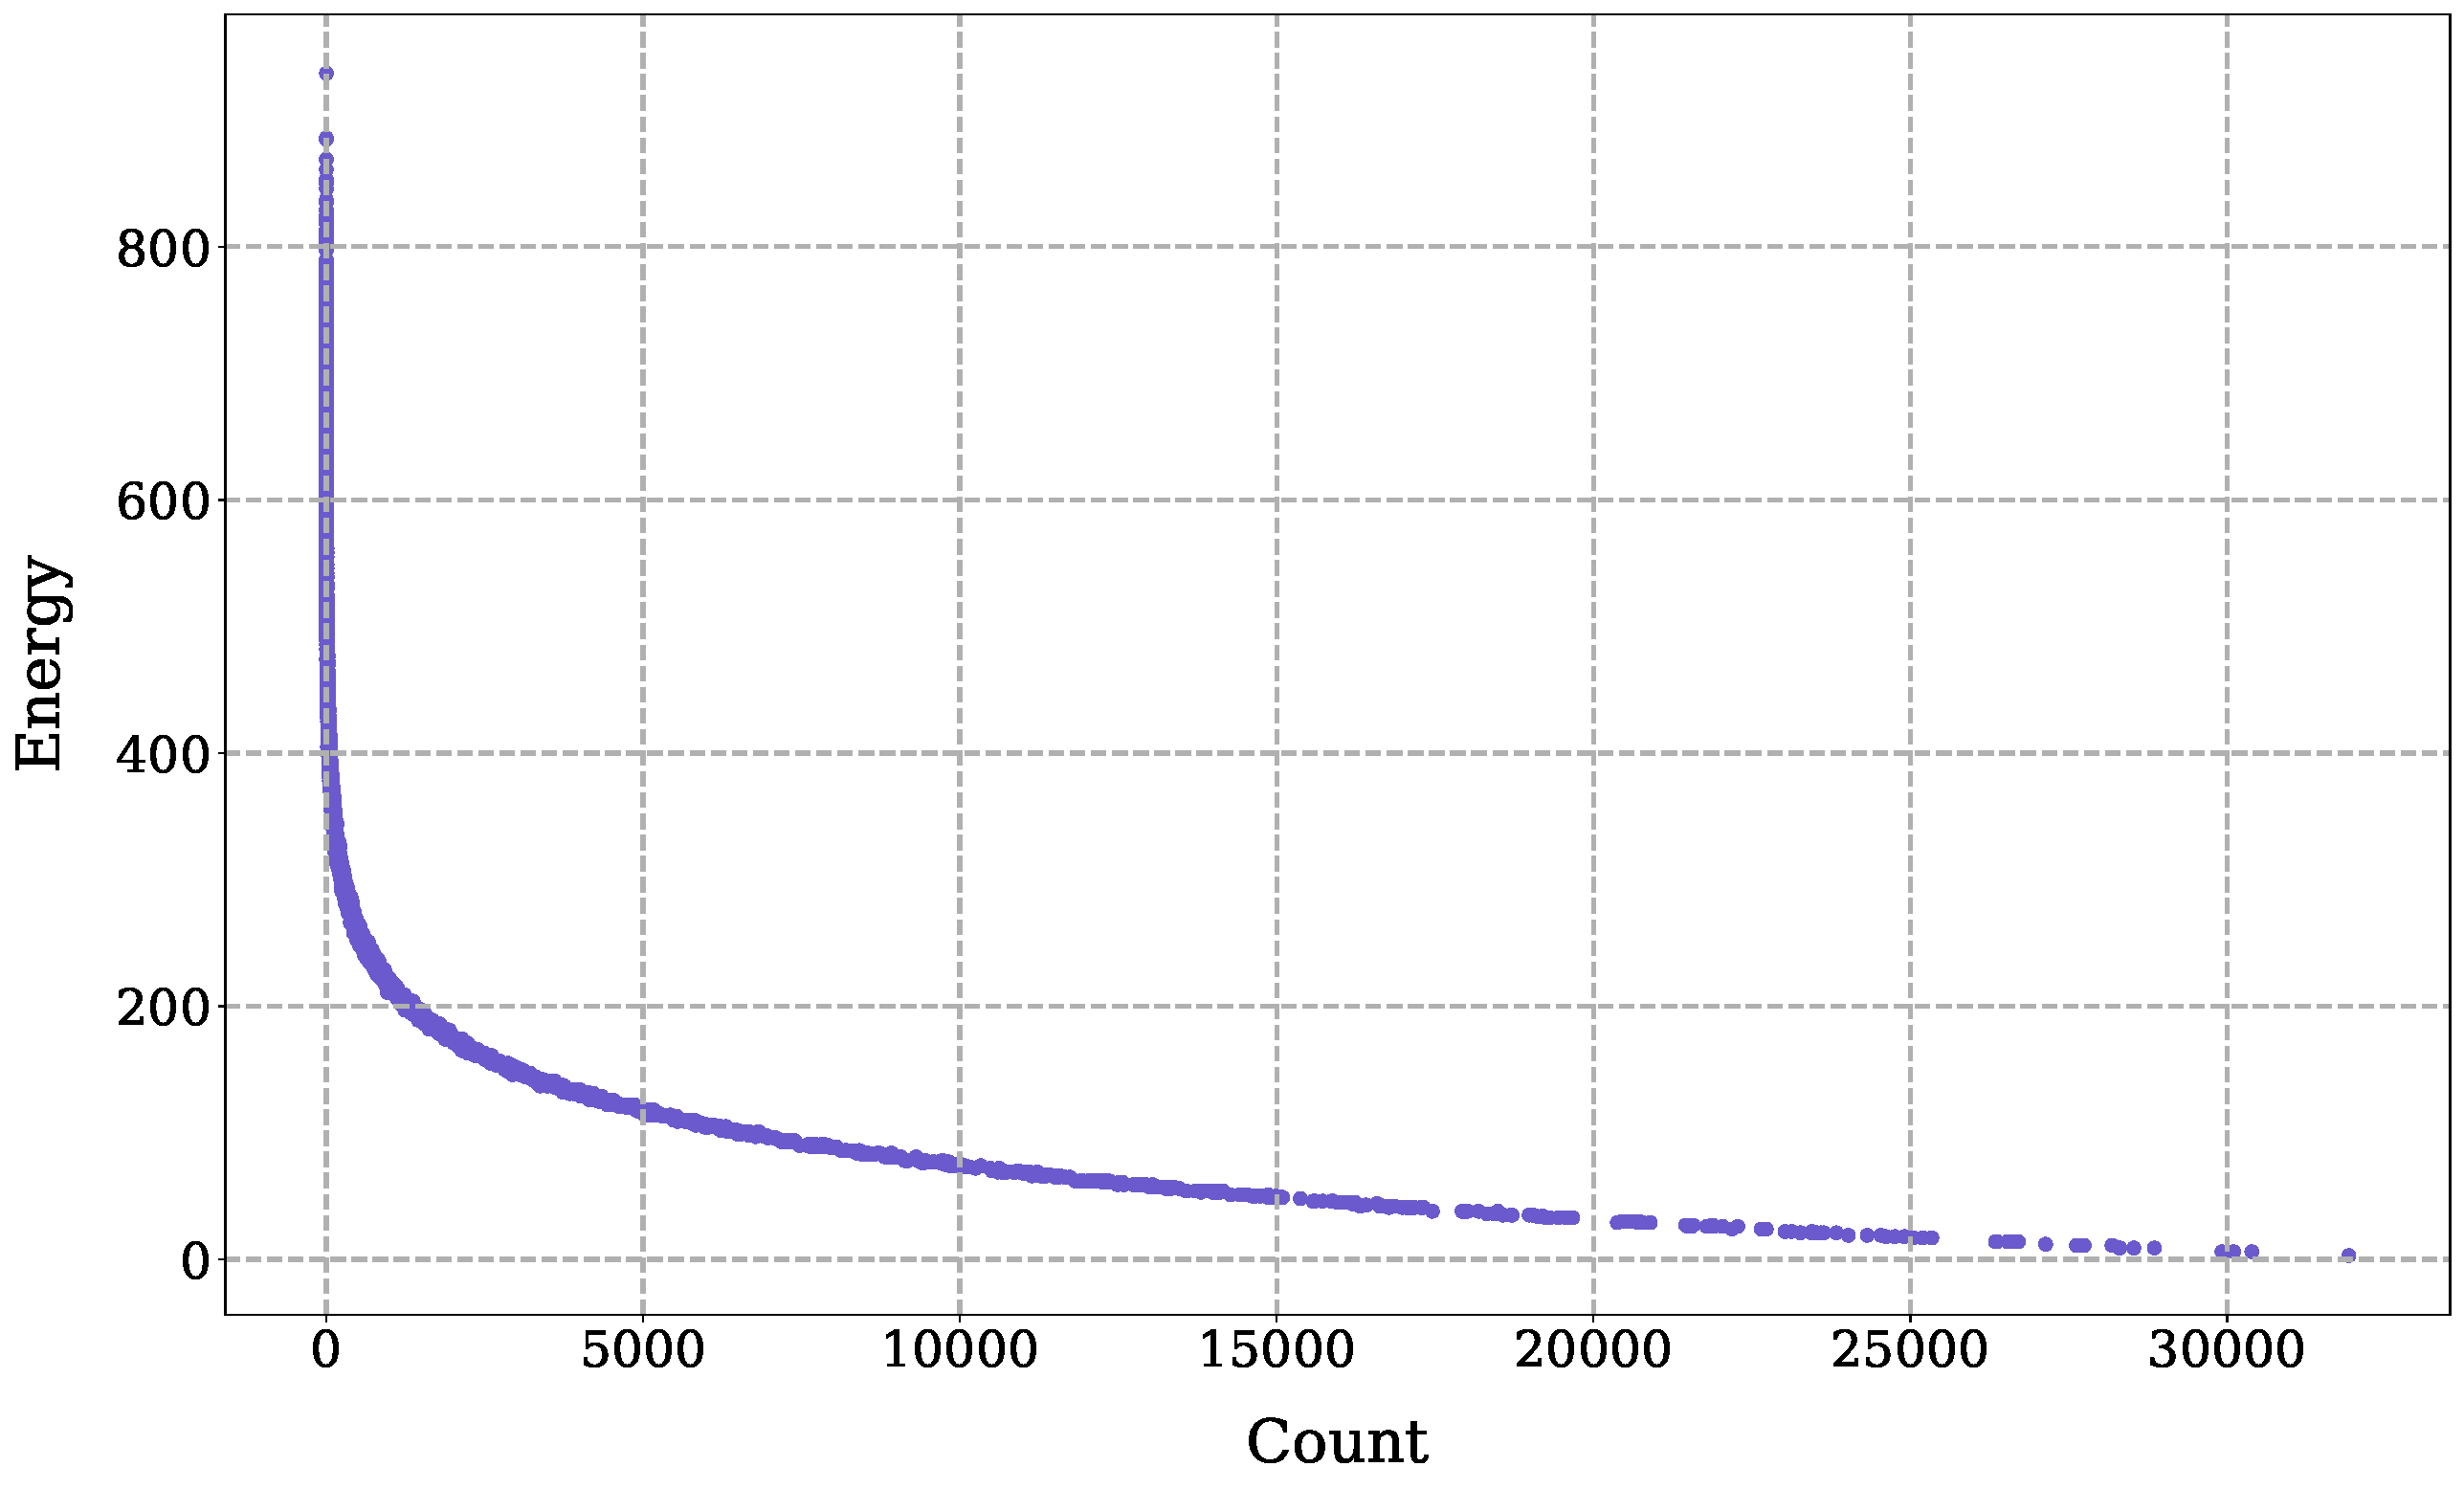
\includegraphics[scale=0.33]{./Figs/IG-scatter.pdf}
	\caption{Energy of the first particle, sharply falling in the beginning, which accounts for the energy distributing over the system, then still falling but in a much more linear manner.}\label{fig:fig7}
\end{figure}

\noindent
From both Figures \ref{fig:fig6} and \ref{fig:fig7} we can see that there are breaking points in the plots, and that has to do with the ways the first particle has to either gain or lose energy - by modifying any of the 3 quantum numbers. From Figure \ref{fig:fig7} though, we can learn that the system still prefers the evenly distributed energy states, and it shows as most of the counts correspond to energy states in the lower fifth of the spectrum.\\\\
Applying logarithm to the values and plotting, we see that there is hardly a linear tendency in the first part of the plot. This, together with the fact that a small displacement is a great error (due to the graph being logarithmic), makes the exponential fitting useless in this case, at least as a single exponential.
\begin{figure}[!h]
	\centering
	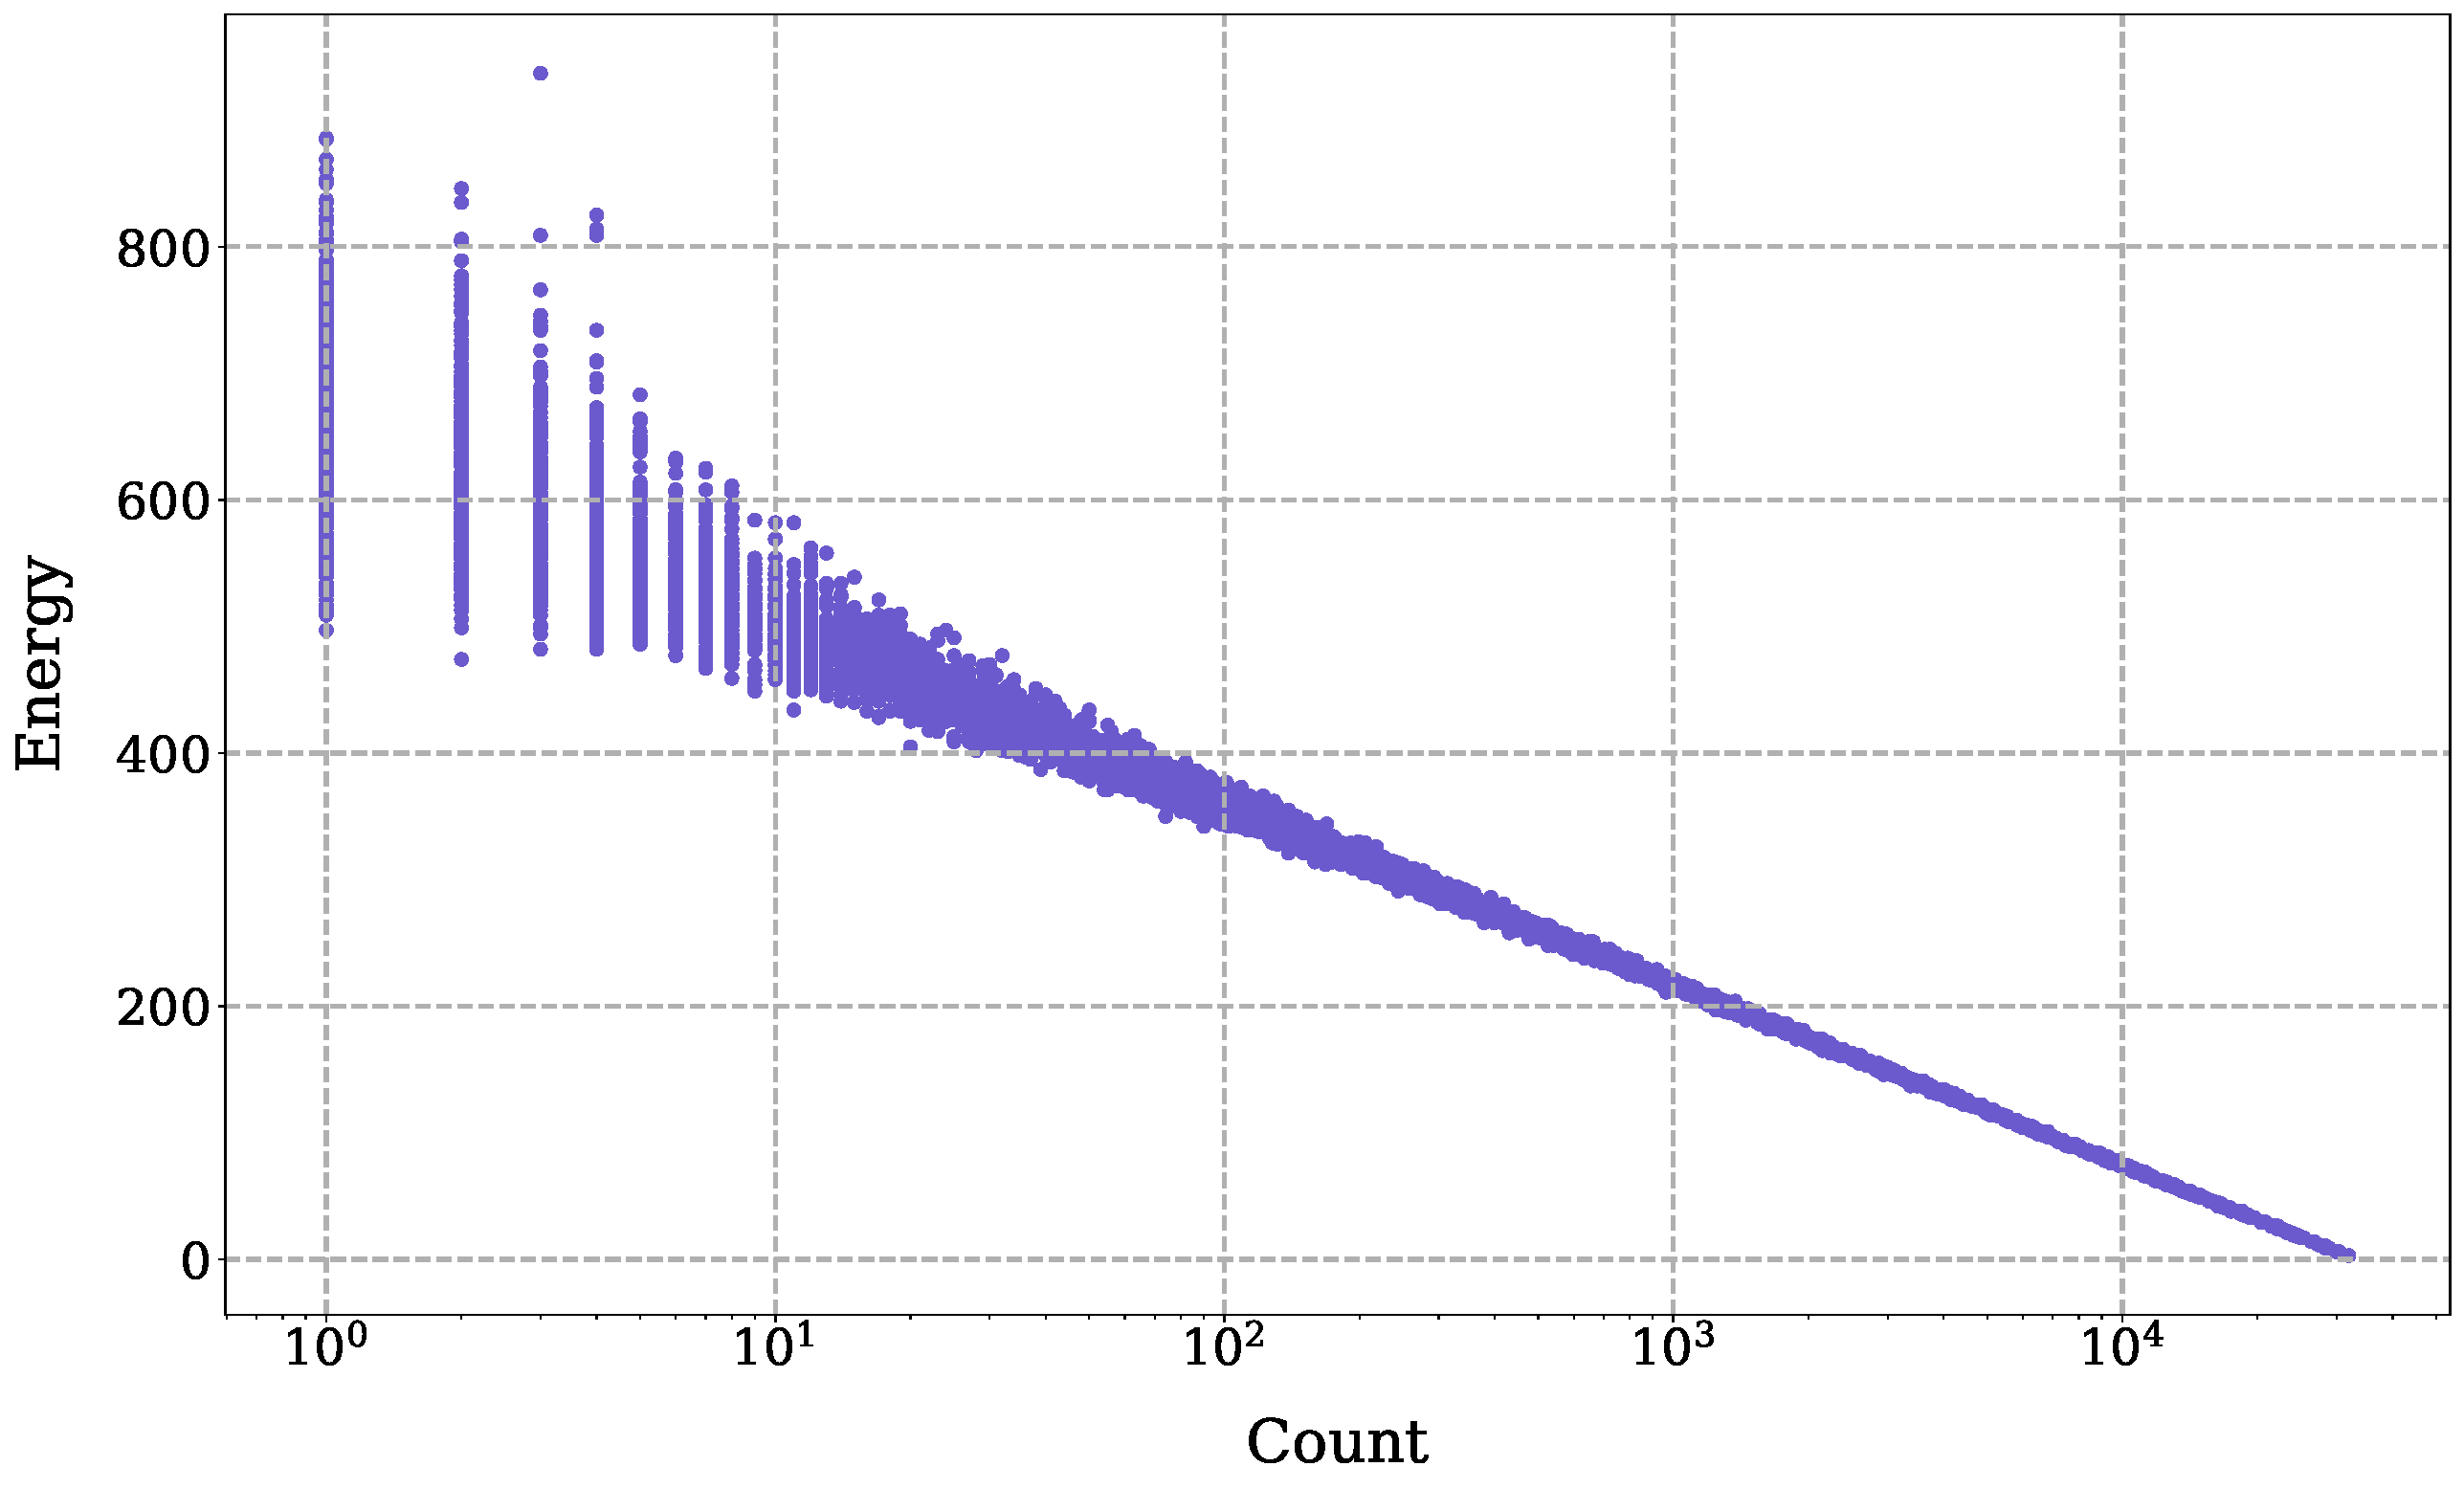
\includegraphics[scale=0.33]{./Figs/IG-scatter-linear.pdf}
	\caption{Energy of the first particle, represented in logarithmic scale ($X$ axis). It is rather hard to make a good fit with an exponential in this case.}\label{fig:fig8}
\end{figure}


\subsubsection*{Conclusions}
We can find similarities between the two experiments performed in this work, owing to the tendency to minimize free energy (which in this case is only energy) and maximize entropy that is natural in thermodynamic systems. However, this assignment also goes to show that there is no ``one size fits all" and we have to be careful in making assumptions when working with thermodynamic systems. So as a final remark, we have seen that there is a balance between achieving the minimum energy state in comparison to the other elements of the system, while at the same time seeking the maximum entropy. Even though these were simple and ideal problems, they are useful to develop a notion in regards to the behavior of coupled or interacting energetic systems.

\end{document}